\documentclass[12pt, a4paper, twocolumn]{report}
\usepackage[utf8]{inputenc}
\usepackage[russian]{babel}
\usepackage{hyperref}
\usepackage[]{graphicx}

%\makeindex

\newcommand{\PROGNAME}{assembly007}

\input{../../commons/doc/style.tex}
\newcommand{\IMPORTANT}{{\bf ВНИМАНИЕ:~}}

\newcommand{\CTL}[1]{<<{\bf #1}>>}

\newcommand{\CMD}[1]{<<{\tt #1}>>}

\newcommand{\FILENAME}[1]{{\tt #1}}

\newcommand{\PARAM}[1]{\item {\bf #1} }

\newcommand{\PARAMSECTION}[1]{\vbox{}{\bf Раздел <<#1>>}}


\title{Установка №~7. \\ Регистрация удельного сопротивления в~зависимости от~температуры с~ручным управлением температурой образца. \\ Руководство пользователя}
\author{Накин~А.~В.}
\date{Версия программы: 2.1\\Ревизия документа: №~3 от \mbox{1 декабря 2016~г.}}

\begin{document}

\maketitle

\tableofcontents

\chapter{Общие сведения}

Установка №~7 (далее~--- Установка) представляет собой программно-аппаратный комплекс для регистрации удельного сопротивления материалов (далее~--- Образцов) в зависимости от температуры.

Установка производит съём показаний измерительных приборов, вычисление значения сопротивления со всеми сопутствующими погрешностями и запись результатов в файлы данных.

Управление температурой Образца производится вручную при помощи:

\begin{itemize}
\item регулируемого трансформатора, питающего обмотку электропечи;
\item манипуляциями со сборкой, например погружением её в пары кипящего азота.
\end{itemize}

Установка сама никак не влияет на температуру Образца, а только регистрирует её вместе с сопротивлением.

Одновременно Установка способна работать только с одним единственным Образцом.

\section{Состав Установки}

\subsection{Состав аппаратной части}

Аппаратная часть Установки состоит из персональной ЭВМ (далее~--- ПЭВМ) и следующих приборов:

\begin{itemize}

\item Мультиметр 34410A/34401A (далее~--- мультиметр) компании Agilent (1--3~шт.). Предназначен для измерения сопротивления Образца (один или два мультиметра) и его температуры посредством измерения напряжения на термопаре. Мультиметры управляются ПЭВМ посредством USB или RS-232 интерфейса.

\item Произвольный источник питания (далее~--- ИП) постоянного тока (0--1~шт.). Предназначен для запитывания электрической цепи с Образцом. Может отсутствовать, если способ измерения сопротивления не требует запитки.

Рекомендуется использовать в качестве ИП Agilent E3645A или аналогичный: в этом случае уменьшается объём ручной работы и, как правило, повышается точность измерений.

\item Измеритель-регулятор одноканальный ТРМ-201 компании ОВЕН (0--1~шт.). Предназначен для определения температуры Образца посредством термопары. Управляется ПЭВМ посредством прибора АС-4, к которому подключён посредством интерфейса RS-485. Может отсутствовать, если для измерения температуры используется вольтметр.

\item Блок из 8-ми управляемых 2-х позиционных реле МВУ-8 компании ОВЕН (1~шт.). Предназначен для коммутации приборов и Образца. Управляется ПЭВМ посредством прибора АС-4, к которому подключён посредством интерфейса RS-485.

\item Преобразователь интерфейсов USB/RS-485 АС-4 компании ОВЕН (1--2~шт.). Предназначен для подключения МВУ-8 и ТРМ-201 к ПЭВМ через USB интерфейс.

\item Эталонное сопротивление (0--1~шт.). Предназначено для измерения тока в цепи посредством измерения падения напряжения на сопротивлении с известным номиналом. Может отсутствовать, если способ измерения сопротивления не требует эталонного сопротивления.

\end{itemize}

\subsection{Состав программной части}
\label{sec_software}

Программная часть Установки состоит из следующих компонентов.

\begin{itemize}

\item Программа Установки (далее~--- Программа), состоящая из нескольких модулей, написанных на языке Tcl.

\item Интерпретатор языка Tcl и необходимые библиотеки. Дополнительные сведения см. в соответствующих документах.

\item Библиотека, предоставляющая программный интерфейс VISA для доступа к приборам 34410A и E3645A. Например: программный пакет IO Libraries Suite компании Agilent. Дополнительные сведения см. в соответствующих документах.

\item Драйвера устройств, подключаемых непосредственно к ПК.


\end{itemize}

\section{Принцип работы}

Установка периодически с заданной частотой измеряет сопротивление и температуру Образца и записывает результаты в файлы, а также выводит на экран ПЭВМ для оперативного контроля. Оператор вручную управляет температурой Образца.

\label{sec_registration_types}

Частота регистрации (записи в файл) измерений вводится оператором перед началом измерений и может задаваться одним из следующих способов:

\begin{itemize}
\item {\bf Временная зависимость}~--- показания регистрируются с фиксированным временным интервалом, например один раз в секунду.
\item {\bf Температурная зависимость}~--- показания регистрируются с фиксированным температурным шагом, например $1$~Кельвин.
\item \label{sec_reg_type_manual} {\bf Вручную}~--- показания регистрируются по команде оператора.
\end{itemize}

\subsection{Определение температуры}

\label{sec_t_measures}

Температура Образца измеряется посредством термопары. Имеется два способа подключения термопары:

\subsubsection*{К вольтметру}

Термопара имеет два спая: рабочий и опорный. Рабочий спай помещается рядом с Образцом, а опорный спай погружается в термостабильную среду с известной температурой (например, жидкий азот). Важно, чтобы температура этой среды не менялась в течении всего эксперимента.

Свободные концы подключаются непосредственно к вольтметру, по показаниям которого определяется разность температур рабочего и опорного спаев.

Данный способ позволяет производить температурные измерения с достаточной точностью (до 0,1~К) и высокой скоростью (до 25~отсчётов в секунду) без потери точности.

\subsubsection*{К ТРМ-201}

Термопара имеет один единственный рабочий спай и подключается к прибору ТРМ-201. Прибор сам определяет температуру <<холодного>> спая (свободных концов термопары), измеряет разность потенциалов на нём и преобразует её в абсолютное температурное значение.

Данный способ возволяет высвободить один мультиметр и не требует наличия термостабильной среды. Недостатки: большая погрешность определения температуры (до 0,5\%) и невысокая скорость измерения (не чаще одного отсчёта в секунду).

\subsection{Определение сопротивления}

\label{sec_r_measures}

Сопротивление Образца измеряется 4-х контактным методом, для чего к Образцу подводятся два потенциальных и два токовых контакта. Сопротивление определяется одним из следующих способов:

\subsubsection{Вольтметром/ амперметром}

Используются вольтметр, амперметр и ИП. Амперметр и ИП включены последовательно с Образцом, амперметр подключён к токовым контактам Образца. Вольтметр включён параллельно с Образцом и подключён к его потенциальным контактам. Сопротивление Образца определяется как $R = V/I$, где $R$~--- искомое сопротивление, $V$~--- показания вольтметра, $I$~--- показания амперметра.

Данный способ наиболее универсальный и точный, но требует максимального количества задействованных мультиметров.

\subsubsection{Вольтметром/ вольтметром}

Используются 2 вольтметра, ИП и эталонное сопротивление номинала $R_2$, включённое последовательно с Образцом и ИП. Первый вольтметр подключён  к потенциальным контактам Образца, второй вольметр --- к выходам эталонного сопротивления. Сопротивление Образца определяется как $R = R_2 V_1/V_2$, где $R$~--- искомое сопротивление, $V_1$~--- показания первого вольтметра, $V_2$~--- показания второго вольтметра.

Данный способ требует максимального количества задействованных мультиметров, а также высококачественное эталонное сопротивление. В ряде случаев он может обеспечить повышенную относительную точность измерений, когда сравниваются результаты измерений одного и того же Образца.

\subsubsection{Вольтметром/ вручную}
\label{sec_voltmeter_manually}

Используются вольтметр и ИП, Образец включён последовательно с ИП, вольтметр подключён к потенциальным контактам Образца. Ток в цепи $I$ считается известным  и неизменным в течении всего эксперимента. Сопротивление Образца определяется как $R = V/I$, где $R$~--- искомое сопротивление, $V$~--- показания вольтметра.

Данный способ наименее точный. Если ИП сам не производит измерение тока в цепи, требуется ручное измерение тока.

\subsubsection{Омметром}

Используется омметр, подключённый к Образцу 4-х контактным способом. Сопротивление Образца определяется непосредственным считыванием показаний омметра.

Данный способ наиболее простой, но не годится в том случае, когда сопротивление Образца слишком мало или велико, то есть выходит за диапазон точных измерений омметра.

\bigskip 

Во всех вышеприведённых способах функции вольметра, амперметра или омметра выполняет мультметр, переведённый в соответствующий режим.


\subsection{Удельное сопротивление}

Установка может самостоятельно вычислять и регистрировать удельное сопротивление Образца по измеренному абсолютному. Для этого перед началом измерений оператор должен ввести параметры Образца. В самом простом случае необходимо ввести только расстояние между потенциальными контактами $l$. Удельное сопротивление тогда вычисляется по формуле:

\begin{equation}
\rho = 2 \pi \cdot R \cdot l,
\end{equation}

\noindent где $\rho$~--- удельное сопротивление, $R$~--- абсолютное сопротивление между потенциальными контактами, $l$~--- расстояние между потенциальными контактами.

Для более точного определения удельного сопротивления необходимо знать поперечное сечение Образца. Для этого оператор должен кроме расстояния $l$ ввести ширину и толщину Образца. При этом предполагается, что Образец имеет форму параллелепипеда, а потенциальные контакты расположены вдоль направления тока. Удельное сопротивление тогда вычисляется по формуле:

\begin{equation}
\rho = \frac{R \cdot w \cdot t}{l},
\end{equation}

\noindent где $\rho$~--- удельное сопротивление, $R$~--- абсолютное сопротивление между потенциальными контактами, $l$~--- расстояние между потенциальными контактами, $w$~--- ширина Образца, перпендикулярная направлению тока, $t$~--- толщина Образца.


\section{Принципиальная схема}
\label{sec_schematic_diagram}

Принципиальная схема Установки приведена на рис.~\ref{pic-scheme}.

Разъёмы J1, J4, J5 расположены на передней панели соединительного бокса. Внутри бокса размещён блок реле МВУ-8, содержащий переключатели S1--S4.

Образец R1 подключён к выходам разъёма J4: токовые контакты к выходам 2 и 6, потенциальные --- к выходам 3 и 7.

Источник питания постоянного тока I1, если используется, подключается к выходам 1, 2 разъёма J5.

Эталонное сопротивление R2, если используется, подключается к выходам 3, 4 разъёма J5.

Мультиметр MM1 может работать:

\begin{enumerate}
\item как вольтметр, измеряя напряжение на потенциальных контактах Образца;
\item либо как омметр, измеряя полное сопротивление Образца; в этом случае мультиметр MM2 не используется, а к выходам 3, 4 разъёма J1 подключены выходы <<Input HI>> и <<Input LO>> мультиметра MM1.
\end{enumerate}

Мультиметр MM2 может работать:

\begin{enumerate}
\item как амперметр, измеряя ток в цепи Образца;
\item как вольтметр, измеряя падение напряжения на эталонном сопротивлении R2;
\item либо отсутствовать.
\end{enumerate}

Полярность подключения мультиметров и ИП не важна.

На схеме изображён способ подключения термопары <<к вольтметру>> (стр.~\pageref{sec_t_measures}). Термопара подключена к выходам 1 и 5 разъёма J4. Напряжение на ней измеряется мультиметром MM3, работающим всегда в режиме вольтметра и подключённого к выходам 5, 6 разъёма J1. Полярность подключения термопары может быть любой, поскольку программная часть Установки может корректировать её показания в случае неправильной полярности.

Если термопара подключена к ТРМ-201, то мультиметр MM3 не используется, а термопара подключается к контактам 4 (<<${}+{}$>>) и 5 (<<${}-{}$>>) разъёма J6. В этом случае полярность подключения играет роль и не может быть изменена программными настройками.

Сдвоенный переключатель S1 предназначен для изменения полярности подключения вольтметра к потенциальным контактам Образца. Сдвоенный переключатель S2 предназначен для изменения полярности подключения ИП в цепь Образца. В данной Установке переключение полярностей не производится.

Переключатель S3 предназначен для размыкания цепи Образца. Размыкание производится:

\begin{itemize}
\item либо в момент переключения полярности посредством S1/S2 во избежание короткого замыкания выходов ИП;
\item либо при измерении сопротивления при помощи омметра, поскольку в данном случае запитка Образца не требуется.
\end{itemize}

Переключатель S4 используется в режиме <<Вольтметром/вручную>> (стр.~\pageref{sec_voltmeter_manually}), когда амперметр MM2 отсутствует: в этом случае S4 переводится в нижнее положение и замыкает цепь питания Образца.

На схеме не изображены ТРМ-201 и подключение блока реле МВУ-8 к внешнему питанию и сети RS-485.

\begin{figure*}
\begin{center}
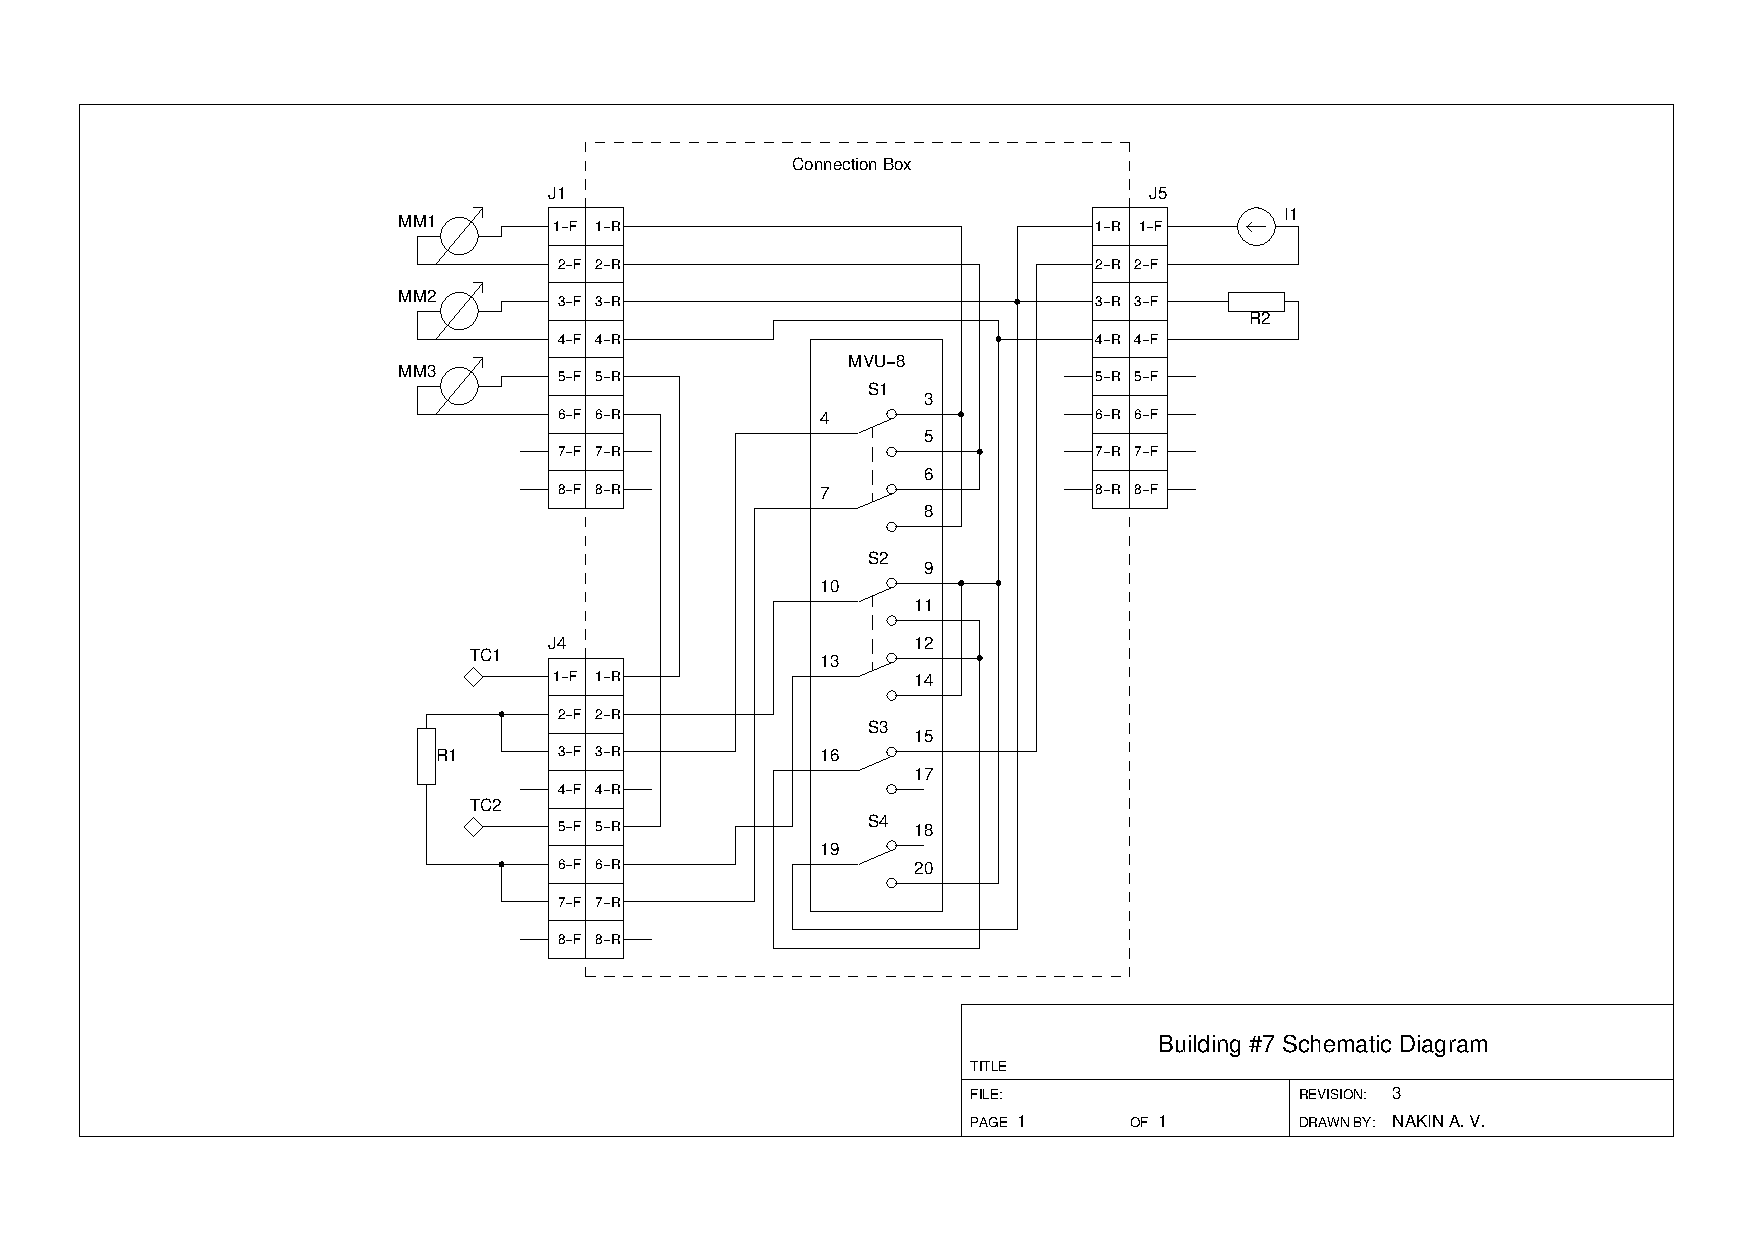
\includegraphics[width=1.0\textwidth, clip, viewport=190 120 630 530]{scheme}
\end{center}
\caption{Принципиальная схема Установки}
\label{pic-scheme}
\end{figure*}

\chapter{Подготовка к работе}

\section{Подготовка аппаратной части}

Включение приборов рекомендуется производить в указанной последовательности.

\subsection{Коммутация мультиметров и ИП}

Соединения внутри соединительного бокса обеспечиваются шлейфом №~6 (далее~--- шлейф).

В зависимости от способа измерения сопротивления измерительные приборы и источник питания подключаются следующим образом:

\subsubsection{Вольтметром/ амперметром}

    \begin{itemize}
        \item Выходы <<Input HI>> и <<Input LO>> мультиметра MM1 подключаются к выходам 1 и 2 разъёма J1. 
        \item Выходы <<Input I>> и <<Input LO>> мультиметра MM2 подключаются к выходам 3 и 4 разъёма J1. 
        \item Выходы источника питания I2 подключаются к выходам 1 и 2 разъёма J5. 
    \end{itemize}

\subsubsection{Вольтметром/ вольтметром}

    \begin{itemize}
        \item Выходы <<Input HI>> и <<Input LO>> мультиметра MM1 подключаются к выходам 1 и 2 разъёма J1. 
        \item Выходы <<Input HI>> и <<Input LO>> мультиметра MM2 подключаются к выходам 3 и 4 разъёма J1. 
        \item Выходы источника питания I2 подключаются к выходам 1 и 2 разъёма J5. 
        \item Тестовое сопротивление R3 подключается к выходам 3 и 4 разъёма J5. 
    \end{itemize}
        
\subsubsection{Вольтметром/ вручную}

    \begin{itemize}
        \item Выходы <<Input HI>> и <<Input LO>> мультиметра MM1 подключаются к выходам 1 и 2 разъёма J1. 
        \item Мультиметр MM2 не используется. 
        \item Выходы источника питания I2 подключаются к выходам 1 и 2 разъёма J5. 
    \end{itemize}
        
\subsubsection{Омметром}

    \begin{itemize}
        \item Выходы <<Input HI>> и <<Input LO>> мультиметра MM1 подключаются к выходам 3 и 4 разъёма J1. 
        \item Выходы <<Sense HI>> и <<Sense LO>> мультиметра MM1 подключаются к выходам 1 и 2 разъёма J1. 
        \item Мультиметр MM2 не используется. 
        \item Источник питания I2 не используется. 
    \end{itemize}


\subsection{Подготовка Образца и термопары}

Подключите Образец, термопару и, возможно, эталонное сопротивление к разъёмам соединительного бокса согласно принципиальной схеме.

\subsection{Подготовка ТРМ-201}

\begin{enumerate}

\item Проверьте подключение устройства к термопаре и источнику переменного напряжения 220~В. Проверьте полярность подключения термопары.

\item Проверьте подключение устройства к устройству АС-4 посредством сети RS-485.

\item Подайте питание на прибор. Должны загореться индикатор <<Питание>> на передней панели прибора и высветиться текущая температура рабочего спая в градусах Цельсия.

\item Устройство должно иметь следующие сетевые настройки:

\begin{itemize}
\item Длина адреса: 8~бит;
\item Скорость: 9600~бод;
\item Чётность: none;
\item Стоповых бит: 1;
\end{itemize}

Сетевые настройки можно установить при помощи программы <<Конфигуратор ТРМ>>, которая идёт в комплекте с устройством. См. документацию к программе для детальных инструкций. Данные настройки, будучи установленными, сохраняются в энергонезависимой памяти устройства и не теряются при отключении питания.

\end{enumerate}


\subsection{Подготовка МВУ-8}

\begin{enumerate}

\item Проверьте подключение устройства к шлейфу и источнику переменного напряжения 220~В;

\item Проверьте подключение устройства к устройству АС-4 посредством сети RS-485.

\item Включите питание соединительного бокса. Должен загореться индикатор <<Питание>> на передней панели прибора.

\item Устройство должно быть настроено на работу по протоколу <<Modbus RTU>>. Согласно <<заводским>> настройкам устройство изначально использует протокол <<ОВЕН>>. Для смены протокола необходимо запустить программу <<Конфигуратор МВУ-8>> и в ней перенастроить устройство. Настройки сохраняются в энергонезависимой памяти и не теряются при выключении питания. То есть будучи настроенным устройство не теряет настроек после выключения и повторного включения питания.

\IMPORTANT Всякий раз при запуске программы <<Конфигуратор МВУ-8>> устройство МВУ-8 автоматически переходит на протокол <<ОВЕН>>. Чтобы вернуть устройство на нужный протокол, нужно выключить его на несколько секунд и включить снова.

См. документацию к программе <<Конфигуратор МВУ-8>> для детальных инструкций.

\end{enumerate}


\subsection{Подготовка АС-4}

Устройство должно быть подключено к ПЭВМ посредством интерфейса USB. На ПЭВМ должен быть установлен драйвер устройства. Если драйвер корректно установлен, в системе должен появиться новый COM-порт, посредством которого программы взаимодействуют с устройствами RS-485, подключёнными к данному экземпляру АС-4.

\IMPORTANT Устройство очень чувствительно к качеству соединения с ПЭВМ, поэтому рекомендуется подключать его непосредственно к USB разъёму ПЭВМ без использования промежуточных USB-разветвителей. Также необходимо использовать качественные USB-кабели с экранированием. В противном случае возможна потеря связи АС4 с ПЭВМ.

\subsection{Подготовка источника питания}

\begin{enumerate}

\item Проверьте подключение измерительных проводов: оно должно соответствовать схеме Установки и режиму измерения.
\item Включите прибор.
\item Установите необходимые в эксперименте значения тока и напряжения.

\end{enumerate}


\IMPORTANT{Если выбран режим ручного измерения тока (см. <<Вольтметром/ вручную>> на стр.~\pageref{sec_voltmeter_manually}), то необходимо установить силу тока в цепи, соответствующую введённому значению. Но если в качестве источника питания используется Agilent E3645A, то программа настроит его самостоятельно, и вмешательство оператора не требуется.} 

\subsection{Подготовка мультиметров 34410A/34401A}

\begin{enumerate}

\item Проверьте подключение измерительных проводов: оно должно соответствовать схеме Установки и режиму измерения.
\item Включите мультиметр. Убедитесь, что он подключён к ПЭВМ.
\item Переведите переключатель <<Front/Rear>> в положение <<Front>> (кнопка отжата). 

\end{enumerate}


\section{Подготовка программной части}

Запустите программу Установки №~7.

Убедитесь в работоспособности Программы и всех аппаратных устройств. Для этого убедитесь, что Программа определяет и выводит на экран ПЭВМ температуру и сопротивления Образца. Откройте вкладку \CTL{Измерение} (она открыта сразу после запуска Программы). В текстовых полях (\CTL{Ток}, \CTL{Напряжение} и т.~д.), а также на графиках должны выводиться обработанные показания приборов. На графике производной температуры по времени $dT/dt$ показания могут выводиться с небольшой задержкой.

После того, как показания приборов начали отображаться на вкладке, убедитесь, что они лежат в ожидаемом диапазоне значений, что говорит о правильности подключения всех устройств и работы Установки. Если некоторые показания явно некорректные, проверьте качество соединений, положение кнопок <<Front/Rear>> мультиметров и пр.

\subsection{Параметры Образца}

Откройте закладку \CTL{Образец}. Данная вкладка содержит параметры измеряемого образца.

\subsubsection{Геометрические параметры}
\label{sec_geom_params}

Если возможно, введите некоторые геометрические параметры. Они будут использоваться для вычисления удельного сопротивления Образца. 

В поле \CTL{Расстояние между потенциальными контактами} введите соответствующее расстояние и его погрешность. В самом простом случае этого достаточно для вычисления удельного сопротивления.

Если образец имеет форму близкую к параллелепипеду, то введите соответствующие размеры в полях \CTL{Длина}, \CTL{Ширина} и \CTL{Толщина}, а также их абсолютные погрешности. При этом длина Образца не используется в расчётах, а ширина и толщина используются для расчёта поперечного сечения.

Допускается, хотя и не рекомендуется, не указывать погрешности геометрических параметров. В этом случае соответствующие поля ввода должны быть пустыми.

Если геометрические параметры Образца неизвестны, очистите все соответствующие поля. В этом случае удельное сопротивление не будет вычисляться автоматически, но на общую работу установки это не повлияет.


\subsubsection{Файлы}

В поле \CTL{Имя файла результатов} вводится путь и имя файла, в который будут записаны результаты измерений для последующего использования. Как правило, это поле обязательно для заполнения. Если поле пустое, то в процессе измерений их результаты не будут фиксироваться в файле, что как правило недопустимо.

Имя файла может включать в себя строчку \CMD{\%AUTODATE\%} (без кавычек). Тогда путь к реальному файлу будет в этом месте включать три
 подкаталога, соответствующих текущим году, месяцу и дню месяца. Например, если в поле введено \CMD{C:\textbackslash{}res\textbackslash{}\%AUTODATE\%\textbackslash{}res.txt}, и измерения проводятся 5 января 2012 года, то реальный путь к файлу будет \CMD{C:\textbackslash{}res\textbackslash{}2012\textbackslash{}01\textbackslash{}05\textbackslash{}res.txt}.

В поле \CTL{Имя файла трассировки} вводится путь и имя файла, в который будут записаны необработанные результаты всех произведённых измерений. Как правило, трассировка нужна только на этапе отладки Установки. Размер файла трассировки значительно превышает размер файла результатов, что может иногда привести к переполнению диска. Так же как и имя файла результатов, имя файла трассировки может включать строку \CMD{\%AUTODATE\%}.

В поле \CTL{Формат файлов} выбирается нужный формат всех создаваемых файлов. В настоящее время поддерживается два формата:

\begin{itemize}
\item \CTL{TXT} --- текстовый формат, в котором каждое измерение записывается в отдельной строке, внутри строки значения разделяются символом табуляции. Формат поддерживается большинством научных приложений.
\item \CTL{CSV} --- текстовый формат, в котором каждое измерение записывается в отдельной строке, внутри строки значения разделяются запятой. Формат поддерживается рядом офисных приложений, например Miscosoft Excel.
\end{itemize}

Флаг \CTL{Переписать файлы} указывает, нужно ли всякий раз в начале измерений переписывать файлы заново. Если флаг сброшен, все новые показания будут дописываться в конец файлов.

В поле \CTL{Комментарий}\label{sec_dut_comment} вводится произвольный фрагмент текста, который будет записан в начале файла результатов. Поле может быть пустым, но рекомендуется вводить в него краткое описание Образца и условия проведения измерений, это в будущем облегчит анализ результатов.


\subsection{Параметры измерения}

Откройте вкладку <<Параметры измерения>>. Содержимое данной вкладки определяет условия проведения измерений.

\subsubsection{Метод регистрации}
\label{sec_reg_method}

В данном разделе выбирается способ и частота регистрации измерений (см. описание принципа работы на стр.~\pageref{sec_registration_types}).

Если требуется регистрация с фиксированным временным интервалом, то выберите флаг \CTL{Временная зависимость}, после чего в поле \CTL{Временной шаг} введите значение интервала.

Если требуется регистрация с фиксированным температурным интервалом, то выберите флаг \CTL{Температурная зависимость}, после чего в поле \CTL{Температурный шаг} введите значение интервала.

Если требуется нерегулярная регистрация, то выберите флаг \CTL{Вручную}.

\subsubsection{Переполюсовка}
\label{sec_switch}

В данном разделе указываются параметры переполюсовки.

Для включения переполюсовки подключения вольметра, отметьте флаг \CTL{Переполюсовка напряжения}.

Для включения переполюсовки подключения источника тока, отметьте флаг \CTL{Переполюсовка тока}.

В поле \CTL{Пауза после переполюсовки} можно указать паузу между окончанием коммутаций и последующими измерениями.

В поле \CTL{Кол-во точек перед переполюсовкой} указывается количество измерений, которое производится при каждой полярности.

\subsubsection{Метод измерения сопротивления}

\label{sec_r_measure_config}

Как было описано в разделе <<Определение сопротивления>> (стр.~\pageref{sec_r_measures}), Установка может определять сопротивление Образца разными способами. В данном разделе указывается нужный способ и вводятся сопутствующие параметры.

Флаг \CTL{Вольтметром/ Амперметром} включает соответствующий метод измерения. Дополнительных параметров в данном случае нет, и напряжение и ток определяются автоматически.

Флаг \CTL{Вольтметром/ Вольтметром} включает соответствующий метод измерения. В данном режиме необходимо ввести номинал эталонного сопротивления и, желательно, его абсолютную погрешность.

Флаг \CTL{Вольтметром/ вручную} включает соответствующий метод измерения.

Флаг \CTL{Омметром} включает соответствующий метод измерения. Дополнительных параметров в данном случае нет, сопротивление определяется автоматически.

В поле \CTL{Сила тока} нужно ввести силу тока в цепи, запитывающей Образец. Значение данного поля используется следующим образом:

\begin{itemize}
\item Если в качестве I1 используется управляемый источник питания, то при начале измерений ему будет послана команда на установления нужной силы тока. Устанавливать её вручную не требуется.
\item Если используется неуправляемый ИП, то введённое значение используется в режиме \CTL{Вольтметром/вручную} ~--- Программа использует его в качестве известной силы тока.
\end{itemize}

В поле \CTL{Погрешность} вводится известная погрешность ИП в регулировании силы тока. Данное значение используется только в режиме \CTL{Вольтметром/вручную} для определения инструментальной погрешности.

\IMPORTANT{При всяком изменении способа определения сопротивления Программа должна быть перезапущена, чтобы изменения вошли в силу.}

\chapter{Измерения}

После подготовки к работе аппаратной и программной частей Установки можно приступить к измерениям.

\section{Проведение измерений}

Выберите вкладку \CTL{Измерение}. Ещё раз убедитесь в том, что все приборы работают, величины температуры и сопротивления Образца измеряются и находятся в ожидаемом диапазоне значений.

После этого нажмите кнопку \CTL{Начать запись}. Установка начнёт регистрацию температуры и сопротивления.

Оператор управляет температурой образца, например увеличением напряжения на обмотке электропечи. Скорость изменения температуры определяется требованиями эксперимента.

Если выбран режим ручной регистрации (стр.~\pageref{sec_reg_type_manual}), то оператор должен самостоятльно нажимать кнопку \CTL{Снять точку}\label{sec_manual} всякий раз, когда требуется зафиксировать измерение.

Кнопка \CTL{Снять точку} доступна и в других режимах, при регистрации временной и температурной зависимостей. То есть даже при автоматической регистрации оператор может вручную зарегистрировать нужное измерение. Например, если выбранный временной интервал довольно велик, а оператор наблюдает <<интересное поведение>> Образца, то он может вручную зафиксировать текущее измерение, даже если временной интервал ещё не истёк.

При необходимости Оператор может заблокировать запись в файл результатов без прекращения измерений. Для этого Оператор должен нажать кнопку \CTL{Приостановить запись}, после чего кнопка останется в <<нажатом>> состоянии. В режиме приостановки записи измерения производятся и отображаются на экране, но не сохраняются в файле результатов. Для возобновления записи оператор должен нажать кнопку повторно.

\IMPORTANT{Если выбран режим ручного измерения тока (см. <<Вольтметром/ вручную>> на стр.~\pageref{sec_voltmeter_manually}), то оператор должен самостоятельно следить за стабильностью силы тока в цепи: его значение не должно отклоняться от введённого заранее значения. В противном случае измерения будут неправильными. Но если в качестве источника питания используется Agilent E3645A, то это ограничение отсутствует, поскольку данный ИП самостоятельно контролирует силу тока. Более того, в процессе измерения допускается изменять силу тока, выдаваемого E3645A, поскольку он также выступает в качестве амперметра и сигнализирует об изменении тока в цепи.} 

По окончании измерений нажмите кнопку \CTL{Остановить запись}, после чего в течении нескольких секунд программа зафиксирует все результаты в файлах. Файлы далее доступны для анализа.

Далее можно произвести новую серию измерений, или завершить работу Установки.

\section{Индикация измерений}

В процессе работы Установка производит снятие показаний приборов, обработку и отображение результатов на экране Программы. Частота, с которой производится опрос приборов, зависит от параметров измерения (см. раздел <<Метод регистрации>> на стр.~\pageref{sec_reg_method}), а также от скорости изменения температуры. Чем быстрее изменяется температура Образца, и чем меньше заданный температурный или временной интервал, чем чаще будут опрашиваться измерительные приборы.

Индикация измерений производится на вкладке \CTL{Измерение}.

\subsection{Диаграммы}

Четыре диаграммы показывают состояние основных регистрируемых величин:

\subsubsection{Зависимость $R(T)$}

На диаграмме изображается зависимость сопротивления Образца от температуры, измерения изображаются в виде зелёных точек, связанных друг с другом. Каждая залёная точка соответствует одному измерению, записанному в файл результатов. Если эксперимент достаточно продолжительный и точек становится слишком много, они автоматически прореживаются, разумеется только на графике.

Кроме того на этой же диаграмме отображается текущее значение сопротивление и температуры в виде небольшого числа сиреневых точек. Эти точки соответствуют промежуточным результатам, которые не подлежат регистрации в файле данных и нужны только для визуального контроля текущего состояния сборки.

\subsubsection{Зависимость R(t)}

На диаграмме изображается зависимость сопротивления Образца от времени, при этом по горизонтальной оси отложено количество измерений (а не время в секундах или иных непосредственных величинах).

Также на диаграмме изображается линейная аппроксимация зависимости $R(t)$ в виде фиолетовой линии. Эта линия даёт возможность оценить тренд изменения сопротивления.

\subsubsection{Зависимость T(t)}

На диаграмме изображается зависимость температуры Образца от времени, по горизонтальной оси отложено количество измерений. Также изображается линейная аппроксимация зависимости $T(t)$ в виде фиолетовой линии.

\subsubsection{Зависимость $\frac{dT}{dt}(t)$}

На диаграмме изображается зависимость скорости изменения температуры Образца от времени, по горизонтальной оси отложено количество измерений. Также изображается линейная аппроксимация зависимости $\frac{dT}{dt}(t)$ в виде фиолетовой линии.

Скорость изменения температуры вычисляется следующим образом. Делается несколько измерений температуры, по ним вычисляется линейная аппроксимация. Скорость изменения температуры определяется как угол наклона этой аппроксимации.

На данном графике значения могут появляться с небольшой задержкой, вызванной тем, что скорость изменения температуры вычисляется спустя некоторое минимальное число измерений.

\subsection{Текстовые поля}

Также индикация измерений производится в текстовых полях, вместе озаглавленных как \CTL{Результаты измерения}. Здесь выводятся следующие текущие значения:

\begin{itemize}
\item ток через Образец;
\item падение напряжения на потенциальных контактах Образца;
\item сопротивление между потенциальными контактами;
\item выделаемая тепловая мощность на Образце между потенциальными контактами (не на всём Образце!);
\item температура Образца и скорость её изменения.
\end{itemize}

Все величины сопровождаются инструментальной погрешностью.

\section{Файл результатов}

В файле результатов в начале идёт строка с комментарием (стр.~\pageref{sec_dut_comment}), далее идут следующие поля:

\begin{enumerate}
\item \CMD{Date/Time} --- местные дата и время, в которое было произведено измерение, в формате \mbox{\CMD{ГГГГ-ДД-ММ чч:мм:сс}}.
\item \CMD{T} --- температура Образца в К.
\item \CMD{+/-} --- погрешность определения температуры в К. Здесь и далее под погрешностью подразумевается абсолютная инструментальная погрешность.
\item \CMD{dT/dt} --- скорость изменения температуры в К/мин.
\item \CMD{I} --- ток через Образец в мА.
\item \CMD{+/-} --- погрешность определения тока в мА.
\item \CMD{U} --- падение напряжения на потенциальных контактах Образца в мВ.
\item \CMD{+/-} --- погрешность определения напряжения в мВ.
\item \CMD{R} --- сопротивление между потенциальными контактами Образца в Ом.
\item \CMD{+/-} --- погрешность определения сопротивления в Ом.
\item \CMD{Rho} --- удельное сопротивление между потенциальными контактами Образца в Ом${}\cdot{}$см. Если геометрические параметры Образца не были указаны (стр.~\pageref{sec_geom_params}), данное поле будет пустым.
\item \CMD{+/-} --- погрешность определения удельного сопротивления в Ом${}\cdot{}$см. Так же как и предыдущее, данное поле будет пустым при невозможности определения удельного сопротивления.
\item \CMD{Manual} --- если данная точка была снята вручную (стр.~\pageref{sec_manual}), в данном поле будет значение \CMD{true}, в противном случае поле будет пустым.
\end{enumerate}

\subsection{Файл с усреднёнными значениями}

Еcли Оператор включил одну или обе переполюсовки (см. раздел <<Переполюсовка>> на стр.~\pageref{sec_switch}), то вместе с основным файлом результатов создаётся файл, в который записываются значения, полученные усреднением измерений в течении одного цикла переполюсовки.

Имя файла с усреднёнными значениями имеет такое же имя и расширение, как у основного файла, но перед расширением добавлен суфикс \CMD{.refined}.

Например, если основной файл результатов называется \CMD{data.txt}, то файл с усреднёнными значениями будет называться \CMD{data.refined.txt}.

\chapter{Завершение работы}

Для завершения работы Установки нажмите кнопку \CTL{Выход} в панели Программы. Программа произведёт сброс всех устройств в исходное состояние и закончит работу. Далее можно приступать к выключению аппаратной части.

\section{Отключение приборов}

Отключение приборов рекомендуется производить в указанной последовательности.

\subsection{Отключение мультиметров 34410A/34401A}

\begin{enumerate}

\item Переведите переключатель <<Front/Rear>> в положение <<Rear>> (кнопка нажата). 
\item Выключите мультиметр.

\end{enumerate}


\subsection{Отключение источника питания}

\begin{enumerate}

\item Установите значения тока и напряжения в минимальные положения.
\item Выключите источник питания.

\end{enumerate}


\subsection{Отключение соединительного бокса}

Выключите питание соединительного бокса.

\bigskip

После этого можно отсоединить приборы и сборку с Образцом.

\chapter{Настройка Программы}

При первом запуске Программы, а также при всяком изменении аппаратной части, требуется произвести настройку или перенастройку программной части, чтобы обеспечить связь с аппаратной частью и, возможно, её калибровку.

\section{Файл конфигурации}

Все свои настройки программа сохраняет в обычном файле с именем \FILENAME{\PROGNAME{}.ini}, который размещается в текущем каталоге. Файл имеет текстовый формат, и при необходимости его можно редактировать в произвольном текстовом редакторе. Если файл конфигурации отсутствует при запуске Программы, он будет автоматически создан.

Обратите внимание: файл конфигурации всегда располагается в {\it текущем} каталоге, а не в каталоге, где расположена сама программа. Эти каталоги могут совпадать, но вообще говоря они могут быть разными. Это позволяет запускать одну и ту же программу, но с разными настройками для разных экспериментов.

Рассмотрим пример. Пусть имеется две измерительные установки, различающиеся, например, сборкой, в которой установлен Образец. Таким образом имеем одинаковый набор мультиметров и источников питания, но в разных экспериментах у нас разные термопары, имеющие разную калибровку. Чтобы каждый раз при переключении не менять настройки, мы делаем следующее:

\begin{enumerate}
\item Создаём два разных каталога, например \FILENAME{C:\textbackslash{}config\textbackslash{}exp1} и \FILENAME{C:\textbackslash{}config\textbackslash{}exp2}.

\item Сама программа путь будет расположена в каталоге \FILENAME{C:\textbackslash{}prog\textbackslash{}assembly007}.

\item Для работы с первой сборкой и переходим в каталог \FILENAME{C:\textbackslash{}config\textbackslash{}exp1} и запускаем программу оттуда. В этом же каталоге будет создан файл конфигурации \FILENAME{\PROGNAME{}.ini}.

\item Для работы со второй сборкой и переходим в каталог \FILENAME{C:\textbackslash{}config\textbackslash{}exp2} и производим аналогичные действия.

\end{enumerate}

Если мы работаем в операционной системе семейства Windows, то удобно будет создать ярлыки для каждой из сборок. В свойствах ярлыка укажите разные рабочие каталоги, тогда при выборе ярлыка будет устанавливаться соответствующий текущий каталог, в котором программа будет искать конфигурационный файл.


\section{Настройка измерения сопротивления}

Откройте вкладку \CTL{Параметры измерения сопротивления} Программы. Здесь оператор вводит параметры (адреса и пр.) устройств, которые используются для определения сопротивления Образца.

\subsection{Блок реле}

В данном разделе --- параметры блока реле МВУ-8, содержащего переключатели S1--S4.

Поскольку данное устройство подключено не к ПЭВМ, а к АС-4, сперва необходимо указать в поле \CTL{Порт для АС-4} имя соответствующего порта.

Далее нужно в поле \CTL{Сетевой адрес МВУ-8} указать адрес устройства сети RS-485, управляемой АС-4. Адресом является целое число в диапазоне 0--248, кратное 8.

Адрес может быть подписан на самом устройстве, в противном случае его можно узнать при помощи программы <<Конфигуратор МВУ-8>>, идущей в комплекте с устройством. Подробную информацию см. в документации к МВУ-8 и программе-конфигуратору.

\IMPORTANT{После работы с конфигуратором устройство МВУ-8 переходит в режим работы с протоколом OWEN. Для возврата на протокол ModBus, поддерживаемый Программой, нужно на несколько секунд обесточить устройство.}

\bigskip

Для проверки правильности параметров можно установить пробное соединение с устройством, для этого нажмите кнопку \CTL{Опрос}. Программа попытается установить связь, после чего сообщит о результатах. Не рекомендуется производить опрос в процессе измерений во избежание потери данных.

\subsection{Вольтметр/омметр на образце}
\label{sec_mm1_config}

В данном разделе --- параметры мультиметра MM1 (см. раздел <<Принципиальная схема>> на стр.~\pageref{sec_schematic_diagram}).

В поле \CTL{Адрес} вводится или выбирается из списка значений адрес устройства. Как правило, если устройство подключено к ПЭВМ и должным образом обнаружено библиотекой VISA, его адрес должен быть в списке.

\bigskip

Если в качестве мультиметра используется Agilent 34401A или аналогичное устройство, подключаемое к ПЭВМ через последовательный интерфейс RS-232, то необходимо указать значения в следующих двух полях.

В поле \CTL{Скорость RS-232} указывается скорость работы последовательного порта. В поле \CTL{Чётность RS-232} указывается способ вычисления контрольной суммы. Эти значения должны совпадать с настройками самого устройства, в противном случае скорее всего связь с ним будет невозможна. Способ настройки см. в документации к мультиметру.

\IMPORTANT{Заводские настройки мультиметра Agilent 34401A следующие: скорость --- \CTL{9600}, чётность --- \CTL{Even}. Эти настройки могут быть изменены, после чего хранятся в энергонезависимой памяти устройства и не теряются при выключении.}

Для мультиметра Agilent 34410A или аналогичного, подключаемого посредством интерфейса USB или GPIB, поля настройки RS-232 должны быть пустыми.

\bigskip

Наконец, поле \CTL{Число циклов 50 Гц на измерение} определяет точность измерений. Мультиметр определяет измеряемую величину не одномоментно, а путём многократных измерений в течении некоторого времени. Если это время кратно продолжительности периода питания сети 220~В, то на результат измерений не будет влиять шум вызванный колебанием питания. Время каждого измерения определяется по формуле:

\begin{equation}
t = N_{50} \cdot 20 \cdot 2,
\end{equation}

\noindent где $t$~--- время в мс, $N_{50}$~--- число циклов, $20$~--- продолжительность одного периода при частоте 50~Гц, $2$~--- коэффициент вызванный тем, что каждое измерение фактически производится дважды: первый раз оно производится для измерения <<нуля>>. Такой способ измерений предотвращает <<уход нуля>> при продолжительных измерениях. Таким образом, при $N_{50} = 1$ продолжительность одного измерения равна $40$~мс, а при $N_{50} = 100$ --- $4$~с.

Согласно документации к мультиметру, при увеличении $N_{50}$ (там этот параметр называется NPLC~--- Number of Power Line Cycles) увеличивается точность измерения. Так, например, при увеличении $N_{50}$ от 1 до 100 абсолютная погрешность измерения постоянного напряжения уменьшается на $\approx 1.5\%$. С другой стороны увеличение $N_{50}$ также увеличивает время измерения, что может быть критичным при высоких скоростях изменения температуры. Подробную информацию о влиянии $N_{50}$ на точность измерений см. в документации к мультиметру.

Рекомендуемое значение параметра~--- 10. Не рекомендуется выбирать в качестве числа циклов дробное значение, поскольку в данном случае результаты измерений будут содержать заметный шум на частоте $50$~Гц.

\bigskip

Для проверки правильности параметров можно установить пробное соединение с устройством, для этого нажмите кнопку \CTL{Опрос}. Программа попытается установить связь, после чего сообщит о результатах. Не рекомендуется производить опрос в процессе измерений, это может привести к потере данных.

\subsection{Амперметр/вольтметр на эталоне}

В данном разделе --- параметры мультиметра MM2 (см. раздел <<Принципиальная схема>> на стр.~\pageref{sec_schematic_diagram}). Способ настройки~--- такой же, как для мультиметра MM1.

\IMPORTANT{Если мультиметр MM2 не используется в схеме Установки (например, при ручном измерении тока), то поле адреса должно быть пустым.}

\subsection{Источник питания}

В данном разделе --- параметры ИП I1 (см. раздел <<Принципиальная схема>> на стр.~\pageref{sec_schematic_diagram}), если в его качестве используется Agilent E3645A или аналогичный.

\IMPORTANT{Если используется ИП другого типа, все поля в данном разделе должны быть пустыми.}

В поле \CTL{Адрес} вводится или выбирается из списка значений адрес устройства. Как правило, если устройство подключено к ПЭВМ и должным образом обнаружено библиотекой VISA, его адрес должен быть в списке.

В поле \CTL{Скорость RS-232} указывается скорость работы последовательного порта. В поле \CTL{Чётность RS-232} указывается способ вычисления контрольной суммы. Эти значения должны совпадать с настройками самого устройства, в противном случае скорее всего связь с ним будет невозможна. Способ настройки см. в документации к устройству.

\IMPORTANT{Заводские настройки Agilent E3645A следующие: скорость --- \CTL{9600}, чётность --- \CTL{None}. Эти настройки могут быть изменены, после чего хранятся в энергонезависимой памяти устройства и не теряются при выключении.}

В поле \CTL{Максимальный ток} указывается максимально возможный ток, который может быть подан в цепь. Поле может быть пустым.

\bigskip

Для проверки правильности параметров можно установить пробное соединение с устройством, для этого нажмите кнопку \CTL{Опрос}. Программа попытается установить связь, после чего сообщит о результатах. Не рекомендуется производить опрос в процессе измерений, это может привести к потере данных.

\section{Настройка измерения температуры}

Откройте вкладку \CTL{Параметры измерения температуры} Программы. Здесь оператор вводит параметры (адреса и пр.) устройств, которые используются для определения температуры Образца.

\subsection{Способ подключения термопары}

В данном разделе оператор выбирает один из способов подключения термопары (см. раздел <<Определение температуры>> на стр.~\pageref{sec_t_measures}).

\subsection{Вольтметр на термопаре}

В данном разделе --- параметры мультиметра MM3 (см. раздел <<Принципиальная схема>> на стр.~\pageref{sec_schematic_diagram}). Способ настройки~--- такой же, как для мультиметра MM1 (стр.~\pageref{sec_mm1_config}). Если для определения температуры используется ТРМ-201, то данный раздел недоступен для редактирования).

\subsection{Измеритель-регулятор ТРМ-201}

В данном разделе --- параметры ТРМ-201, используемого для определения температуры. Если для определения температуры используется вольтметр, то данный раздел недоступен для редактирования).

Поскольку данное устройство подключено не к ПЭВМ, а к АС-4, сперва необходимо указать в поле \CTL{Порт для АС-4} имя соответствующего порта.

Далее нужно в поле \CTL{Сетевой адрес ТРМ-201} указать адрес устройства сети RS-485, управляемой АС-4. Адресом является целое число в диапазоне 0--248, кратное 8.

Адрес может быть подписан на самом устройстве, в противном случае его можно узнать при помощи программы <<Конфигуратор ТРМ>>, идущей в комплекте с устройством. Подробную информацию см. в документации к устройству и программе-конфигуратору.

\bigskip

Для проверки правильности параметров можно установить пробное соединение с устройством, для этого нажмите кнопку \CTL{Опрос}. Программа попытается установить связь, после чего сообщит о результатах. Не рекомендуется производить опрос в процессе измерений во избежание потери данных.

\subsection{Термопара}

В данном разделе --- параметры термопары, используемой для определения температуры Образца.

В поле \CTL{Тип термопары} выбирается один из поддерживаемых типов. Расшифровку типов термопар см. в таблице~\ref{tab_tc_types}

\begin{table*}
\begin{center}
\caption{Типы термопар}
\begin{tabular}{cl}
\hline \hline
B & Платина 30\% + Родий / Платина 60\% + Родий (ТПР) \\
C & Вольфрам 5\% + Рений / Вольфрам 26\% + Рений \\
E & Хромель / Константан (ТХКн) \\
J & Железо / Константан (ТЖК) \\
K & Хромель / Алюмель (ТХА) \\
L & Хромель / Копель (ТХК) \\
N & Нихросил / Нисил (ТНН) \\
R & Платина 13\% + Родий / Платина (ТПП13) \\
S & Платина 10\% + Родий / Платина (ТПП10) \\
T & Медь / Константан (ТМКн) \\
\hline \hline
\end{tabular}
\label{tab_tc_types}
\end{center}
\end{table*}

В поле \CTL{Опорная температура} вводится температура опорного спая термопары, которая считается постоянной на всём протяжении эксперимента. Например, если опорный спай погружён в жидкий азот, поле должно иметь значение $77.4$. Если термопара подключается к ТРМ-201, то опорный спай отсутствует и данное поле недоступно для редактирования.

Флаг \CTL{Инв. полярность} меняет полярность подключения термопары к вольтметру. Если температура, отображаемая Программой, некорректная (слишком большая или слишком маленькая), это может быть вызвано тем, что термопара подключена с неправильной полярностью. Менять физическое подключение в этом случае не нужно, достаточно поменять значение флага на противоположное. Если же термопара подключается к ТРМ-201, то программа не может самостоятельно менять полярность, и данное поле недоступно для редактирования. В этом случае оператор должен соблюдать правильную полярность при физическом подключении термопары к ТРМ-201.

В поле \CTL{Выражение для коррекции} вводится арифметическое выражение, которое меняет некоторым образом температуру, полученную непосредственно от термопары. Как известно, всякая термопара требует калибровки, по результатам которой показания должны быть скорректированы для устранения систематической погрешности. В данном поле и вводится это выражение для коррекции.

Выражение включает в себя переменную, которая содержит в себе температуру, полученную непосредственно от термопары, одно или несколько чисел и арифметические операции, выражаемые символами \CMD{+}, \CMD{-}, \CMD{*} и \CMD{/}. Порядок операций~--- как принято в арифметике, для изменения порядка используются круглые скобки. Переменная обозначается произвольной латинской буквой. Между операндами допускается произвольное количество пробелов для улучшения читабельности.

{\bf Пример. } Пусть показания термопары дают температуру, увеличенную на $0.5$~К по сравнению с реальной, корректировка должна уменьшать исходное значение на $0.5$. Тогда выражение для корректировки будет \mbox{\CMD{x - 0.5}} (выражение вводится в поле без кавычек).

\bigskip

Для облегчения калибровки Программа может автоматически составить выражение для коррекции по двум контрольным измерениям температуры:

\begin{enumerate}
\item Нажмите кнопку \CTL{Калибровка}, откроется окно \CTL{Калибровка термопары}.
\item Погрузите рабочий спай термопары в первую среду с известной температурой.
\item Введите в строке \CTL{Температурная точка №~1} в колонке \CTL{Ожидаемая} температуру первой среды в кельвинах. Например, для кипящего азота введите значение \CMD{77.4}, для тающего льда~--- \CMD{273.15}.
\item Ориентируясь на показания температурного графика дождитесь момента, когда температура рабочего спая придёт в равновесие, после чего нажмите кнопку \CTL{Снять} напротив первой температурной точки. Показания термопары будут сниматься в течении некоторого времени для более высокой точности калибровки.
\item По окончании измерения первой точки погрузите рабочий спай термопары во вторую среду с известной температурой.
\item Введите в строке \CTL{Температурная точка №~2} в колонке \CTL{Ожидаемая} температуру второй среды.
\item Аналогичным образом дождитесь момента, когда температура рабочего спая придёт в равновесие, после чего нажмите кнопку \CTL{Снять} напротив второй температурной точки.
\item По окончании контрольных измерений нажмите кнопку \CTL{Сохранить}.
\end{enumerate}

Программа вычислит подходящее выражение для коррекции и запишет его в поле. После этого оператор может в случае необходимости вручную изменить это выражение.

\section{Завершение настройки}

По окончании настройки Программа должна быть перезапущена, чтобы именения вошли в силу.

\chapter{Устранение неиправностей}

\section{Общие рекомендации}

Если при запуске Программы результаты измерений не отображаются, то рекомендуется выполнить следующие действия:

\begin{enumerate}
\item Убедитесь в правильности всех подключений.
\item Убедитесь, что выбранный в Программе метод измерения (стр.~\pageref{sec_r_measure_config}) соответствует схеме Установки и подключениям.
\item Убедитесь, что Программа установила связь со всеми устройствами. Для этого зайдите на вкладку \CTL{Параметры установки} и выполните опрос всех используемых устройств по очереди.
\end{enumerate}

В случае обнаружения неверных настроек (например, выбран неверный метод измерения или введён неправильный адрес устройства), выполните их коррекцию и перезапустите Программу.

Если все вышеуказанные действия не помогли, необходимо ознакомиться с содержимым файла протокола для детального выяснения неисправности.

\section{Файл протокола}

Программа записывает информацию о всех обнаруженных неисправностях аппаратной части в файл протокола с именем \FILENAME{\PROGNAME{}.log}, который размещается в текущем каталоге. Файл всегда пополняется, то есть при обнаружении ошибки новые записи добавляются в конец файла.

Файл имеет простой текстовый формат, в котором каждая запись имеет следующий вид:

\CMD{Время Важность Модуль Описание}

Здесь <Время>~--- точные дата и время обнаружения неисправности. <Важность>~--- важность ситуации, которая может принимать следующие значения:

\begin{itemize}
\item \CTL{critical} --- критическая ошибка;
\item \CTL{error} --- важная ошибка;
\item \CTL{warning} -- предупреждение о возможной ошибке;
\item \CTL{info} --- информационное сообщение, не сигнализирующее об ошибке;
\item \CTL{debug} --- отладочное сообщение, предназначенное для отладки программы.
\end{itemize}

<Модуль>~--- имя модуля Программы, в котором обнаружена ошибка. <Описание>~--- произвольное текстовое описание, детально раскрывающее суть и местоположение ошибки. Описание может распологаться на нескольких строках файла протокола.

Если файл протокола отсутствует при работающей программе, значит в процессе работы ещё не возникало ни одной ошибки.

Файл протокола можно безопасно удалять, он будет вновь создан при первой же возникшей ошибке.

Поскольку файл протокола постоянно пополняется, оператору следует время от времени удалять его во избежание переполнения диска.


\end{document}
